\documentclass[twocolumn]{article}
\usepackage{graphicx}
\usepackage{url}
\usepackage{hyperref}


\begin{document}

\title{Making an 8k Low-resolution Graphics Demo for the Apple II}
\author{DEATER, AKA Vincent M. Weaver}
\date{}
\maketitle

\section{Why would anyone do this?}

I was making an inside-joke filled game for my retro system of choice,
the Apple II.
This involves a Final-Fantasy flying-over-the-planet scene, and while
I was originally going to fake this I found that it was just barely
possible to achieve this in real time.

Once I got it working I realized this would be great as part of a
graphics demo, so off on that tangent I went.
This despite the fact that all I know about the demoscene I learned
from a few viewings of the Future Crew Second Reality Demo plus some
dimly remembered Commodore 64 and Amiga flamewars from a few decades ago.

%  This started out as some SNES style mode7 pseudo-3d graphics code
%  I came up with while working on my TF7 game.  The graphics looked
%  pretty cool, so I started developing a demo around it.

To make thins even better, the code ended up being roughly around 8kB so a
lot of time was wasted fitting it under that arbitrary size limitation.

So in the end this ends up being impressive mostly because so few people
have bothered to write demos for this particular platform.
Though I must make a shout out to the FrenchTouch group whose Apple II
demos put this one to shame.

%  The codesize ended up being roughly around 8kB, so I thought I'd
%  make it into an 8k demo.  There aren't many out there for the Apple II.
%  and a Mockingboard sound card.

%  The demo tries to hit the lowest common denominator for Apple II systems,
%  so in theory you could have run this on an Apple II in 1977 if you
%  were rich enough to afford 48k of RAM.  The Mockingboard sound wasn't
%  available until 1981, but still this all predates the Commodore 64.

%I was writing a game for the Apple II and realized I had come up with
%some clever Super-Nintendo (SNES) style graphics routines that were just
%crying to be turned into a demo-scene style demo.

%The Apple II was the first computer I had access too, and I grew up in an odd
%neighborhood where it was all Apples and not a Commodore to be seen.
%My family long ago got rid of our machine, but I rescued an Apple IIe platinum
%from the dumpster one day and have dragged it from state to state ever since.

%I find 6502 assembly to be oddly therapeutic, and will code in it when other
%projects become too stressful.  Especially when Linux up and hangs on me
%because firefox tried to do something stupid in javascript.  I then pine for
%the days when you could do something useful in 64k of RAM, and not have your
%machine fall over because somehow 4GB is not enough.

%Background:

%The Apple II was the first computer I programmed on, lo many years ago.
%Mostly in Applesoft BASIC (which ended up being the only Microsoft product
%I ever liked) but I was starting to get into assembly language about the
%time my family got a 386 system.

%I've revisited over the years, with some 6502 programming to show I could.
%My skills were not that great, I had one of my size-optimization projects
%crowd re-optimized.  For a while I had a side-gig re-optimizing modern games
%in BASIC, before getting sidetracked into going full in on 6502 assembly
%again.

%Introduced in 1977.
%The Apple II runs at 1.XX check Megahertz.  6502, which can easily
%address 64 kB of RAM (more with bank switching).  Shipped with as little
%as 4kB of RAM.  Three registers, (A,X,Y) but a large ``zero page'' which
%gives you register-like actions on the first 256 bytes of RAM.
%
%DOS3.3 operating system with 140k floppies.  Amazing programming by Wozniak,
%allowing all kinds of floppy protection shenanigans (cite 4am, previous
%article).

\section{The Hardware}

	The Apple II was introduced in 1977.
	This demo should run on an original system, though I do not
	have hardware that old to test on.
	Note this predates the Commodore 64 by five years.

	{\bf CPU, RAM and Storage}

	The Apple II has a 6502 processor running at roughly 1.023MHz.

	Early models only shipped with 4k of RAM, but later 48k, 64k, and 128k
	systems were common.
	The demo requires 48k; this would have been very expensive in 1977.

	Also in 1977 you would probably be loading this from cassette tape, as
	it would be another year before Woz's 140k (single-sided)
	$5\frac{1}{4}$" Disk II came about.
	
	{\bf Sound}

	The only sound available is a bit-banged speaker.
	There was no timer interrupt,
	if you wanted music you had to cycle-count via the CPU.

	This demo uses the Mockingboard soundcard which was introduced in
	1981.  This board is extremely simple, with dual AY-3-8910 sound
	chips controlled by 6522 I/O chips.
	Each chip provides 3 channels of square waves, with noise and
	envelope effects available.

	{\bf Graphics}

	The Apple II had nice graphics for its time, with this time being
	around 1977.  Otherwise it is quite limited.

	\begin{center}
	\begin{tabular}{|c|c|}
	\hline
	Hardware Sprites     &	No \\
	Linear framebuffer   &	No \\
	User-defined charset &	No \\
	Blanking interrupts  &	No \\
	Palette selection    &	No \\
	Hardware scrolling   &	No \\
	Hardware page flip   &	Yes \\
	\hline
	\end{tabular}
	\end{center}

	The hi-res graphics mode was a complex mess of NTSC hacks by Woz.
	You got 280x192 graphics, with 6 colors available.  However the colors
	were from NTSC artifacts and there were limitations on which colors
	could be next to each other (in blocks of 3.5 pixels) as well as
	fringing.  Also the addresses were interleaved, so not a linear
	framebuffer.  Hi-res page0 is at
	\$2000\footnote{On 6502 systems hexadecimal values are 
	indicated by the dollar sign}
	 and page1 at \$4000.
	Optionally 4 lines of text can be shown at the bottom of the
	screen instead of graphics.

	The lo-res mode is a bit easier to use.  It is 40x48 blocks
	(40x40 if 4 lines of text are displayed at the bottom).
	15 colors are available, though there is fringing at the edges.
	Again the addresses are interleaved.  Lo-res page0 is at \$400
	and page1 is at \$800.

	Some amazing effects can be achieved by cycle counting, reading
	the floating bus, and racing the beam while toggling graphics
	modes on the fly.
	Unfortunately for you this demo does not do any of those things
	so you will not be reading about that today.

%Later models added double low-res (80x48) and double hi-res (x y in
%NTSC 15 color) but didn't appear until 198x, and only on later IIe, IIc
%models.

%Apple also came out with the IIgs which arguably was much more advanced
%and cheaper than the Mac, but Apple cancelled the II line much to the
%sadness of the users (Apple II forever).


\section{Setup Ramblings}

I do my development on Linux, using the nano text editor.  I use the
ca65 assembler from the cc65 project, which I find to be a reasonable
tool although most ``real'' Apple II programmers look down on it for some
reason.

I cross-compile on x86 Linux, construct Apple DOS33 disk images using
some tools I've written, and then do most testing in an emulator.
(These days usually AppleWin under the wine emulator, or else MESS/MAME
which has cleaner sound output).  Once things work then I'll stick things
on a USB stick and transfer to the CFFA3000 disk emulator installed in
the actual Apple II.

%\section{Related Work}
%
%See anything by the group FrenchTouch, whose Apple II demos outclass
%mine by a lot.


%  http://www.deater.net/weave/vmwprod/mode7_demo/




\section{The Demo}

\subsection{BOOTLOADER}

   An Applesoft BASIC "HELLO" program loads the binary.
   This just makes things auto-boot at startup, this doesn't count
   towards the executable size, you could manually BRUN the 8k program
   if you wanted.

   The binary is loaded at \$2000 (hi-res page0) and BASIC kicks into
   HIRES mode before loading so you can watch as the memory is loaded
   from disk in a seemingly random pattern.

   Since this is an 8k demo, the entirety of the program is shown on
   the screen (or would be if we POKEd the right address to turn off
   the 4 lines of text on the bottom of the screen).

   Execution starts at address \$2000

\subsection{DECOMPRESSER}


   The binary is LZ4 encoded.  The decompresser flips to HGR page 1 so
   we can watch memory as the program is decompressed.

   The LZ4 decompression code was written by qkumba (Peter Ferrie).
	http://pferrie.host22.com/misc/appleii.htm

   The actual program/data decompresses to around 22k starting at \$4000.
   It over-writes parts of DOS3.3, but since we won't be using the disk 
   anymore this isn't an issue.

   At the top left corner of the screen you'll see the VMW triangles logo
   as it decompresses.  To do this I had to put the proper bit pattern
   at \$4000, \$4400, \$4800, and \$4C00.  I mean to have some words too
   but ran out of disk space.  The bit pattern at \$4000 is executable
   and is run as code.

   Optimizing for code size inside of a compressed binary is a pain.
   Removing instructions sometimes made the binary larger as it no longer
   compressed as well.  Long runs of values (such as 0 padding) are 
   essentially free.  This was a difficult challenge.

\subsection{FADE EFFECT}

  The title screen fades in from black.

  This is a software hack, with a lookup table copying from an off-screen
  buffer.  The Apple II doesn't have any palette support.

\subsection{TITLE SCREEN}

   Once things are decompressed, we jump to \$4000.  We switch to low-res
   mode for the rest of the DEMO.

   A background image is loaded from disk.  This is RLE encoded (probably
   unnecessary when being further LZ4 encoded).

   Why not just load the program at \$400 and load the graphics image for
   free?  Well, remember the graphics are 40x48 (shared with the text).
   Really it's 40x24, with each text char mapping to 4-bits top/bottom
   for color.  Do the math, we have 1k reserved for this mode but 40x24
   is only 960 bytes.  It turns out there are "holes" in the address range
   that aren't displayed, and various pieces of hardware use these holes
   as scratchpad memory.  So if you just blindly uncompress graphics data
   there you can corrupt the scratchpad.  So you have to be careful
   when uncompressing to skip the holes.

   The title screen has scrolling text at the bottom.  This is nothing fancy,
   the text is in a buffer off screen and a 40x4 chunk of RAM is copied in
   every so many cycles.

   You might notice that there is tearing/jitter in the scrolling, even
   though we are double-buffering the graphics.  This is because there is
   not a reliable cross-platform way to get the VBLANK info (especially
   on older machines) so we are having some bad luck about when we flip
   pages.

\subsection{MOCKINGBOARD MUSIC}

   I like chiptune music, especially that for AY-3-8910 based systems.
   Before obtaining a Mockingboard I built a Raspberry Pi chiptune player
   that is essentially the same hardware.

   Most of my sound infrastructure involves YM5 files, which are often used
   by ZX Spectrum and ATARI ST users.  These are usually register dumps
   taken typically at 50Hz.  So to play them back you just have to interrupt
   50 times a second and write the registers.

   To program the Mockingboard, each AY-3-8910 chip has 14 sound related
   registers that control the 3 channels.  Each AY chip has a dedicated
   VIA 6522 parallel I/O chip that handles the I/O.

   Doing this quickly enough is a challenge on the Apple II.  For each
   register you have to do a handshake, set the register \# and the value.
   This can take upwards of 40 1MHz cycles per register.

   For complex chiptune files (especially those written on an ST with much
   faster hardware) it's sometimes not possible to get exact playback
   due to the delay.  Also one AY is on the left channel and one on the right
   so you have to write both if you want sound from both speakers.

   I have a whole suite of code for manipulating YM sound data, in my
   vmw-meter git repository.

   The first step for getting this to work is detecting if a mockingboard is
   there.  This can be in any slot 1-7 on the Apple II, though typically
   Slot 4 is standard (in this demo we only check slot 4).

   The board is initialized, and then one of the 6522 timers is set to
   interrupt at 25Hz (it has to be an on-board timer as the default
   Apple II has no timers).

   Why 25Hz and not 50Hz?  At 50Hz with 14 registers you use 700 bytes/s.
   So a 2 minute song would take 84k of RAM, much more than is available.

   For this demo I run at 25Hz, and also pack the 14 registers of the data
   into 11 (there are various fields that are not packed well, we can
   unpack at play time).  Also I stripped out the envelope data as many
   songs do not use it (so this is a lossy compression method).

   Also, we keep track of the last values written last frame and only
   write out to the board if things change, which helps with the latency
   a bit.

   The sound quality suffered a bit, but it's hard to fit a catchy chiptune
   file in 8K.

   The song being played is a stripped down and re-arranged version of
   "Electric Wave" from CC'00 by EA (Ilya Abrosimov). 


\subsection{MODE7 BACKGROUND}

  "MODE7" was a Super Nintendo (SNES) graphics mode that took a tiled
  background and transformed it to look as if it was squashed out to
  the horizon, giving a 3d look.  The SNES did this in hardware, but
  in this demo we do this in software.

  As found on Wikipedia, the transform is of the type

  [x'] = [a b]([x]-[x0])+[x0]
  [y']   [c d]([y] [y0]) [y0]
  
  For our code, we managed to reduce things to a small number of additions
  and subtractions for each pixel on the screen.  Of course the 6502 can't
  do floating point, so we do fixed point math.  We convert as much as we
  can to table lookups that are pre-calculated.  We also make liberal use
  of self-modifying code.

  Despite all of this there are still some cases where we have to do a 
  16bit x 16bit = 32bit multiply, something that is *really* slow on 6502,
  around 700 cycles (for a 8.8 x 8.8 fixed point multiply).

  To make this faster we use a method described by Stephen Judd.

  The key to note is that $(a+b)^{2} = a^{2}+2ab+b^{2}$ 
	and $(a-b)^{2}=a^{2}-2ab+b^{2}$
  and if you add them you can simplify to:
	$a\times b =\frac{(a+b)^{2}}{4} - \frac{(a-b)^2}{4}$

  This is you have a table of squares from 0..511 (all 8-bit a+b and a-b
  will fall in this range) then you can convert a multiply into a table
  lookup plus a subtract.

  The downsize is you will need 2kB of squares lookup tables (which can
  be generated at startup).  This reduces the multiply cost to the order
  of 200 to 250 cycles.

  By using the fast multiply and a lot of careful optimization you can
  generate a Mode7 background in 40x40 graphics mode at about 5 frames/second.

  The engine can be parameterized with different tilesets to use, which we
  do to provide both a black+white checkerboard background, as well as the
  island background from the TFV game.

\subsection{BOUNCING BALL ON CHECKERBOARD}

  What would a demo be without some sort of bouncing geometric shape.

  This is just done with 16 sprites.  The sphere was modeled in OpenGL
  from a 2000-era game-engine that I never finished.  I then took screenshots
  and then reduced the size/color to an appropriate value.

  The shadow is also just sprites.

  The clicking noise on bounce is just touching the speaker at \$C030.
  It's mostly there to give some sound effects for those playing the demo
  without a mockingboard.

\subsection{TFV SPACESHIP FLYING}

  The spaceship, water splash, and shadows are all sprites.  This is all
  done in software, the Apple II has no sprite hardware.

  This is the TFV game engine flying-spaceship code, with the keyboard
  routines replaced to read from memory instead (sort of like a script
  of what to do when). 

\subsection{STARFIELD}

  The starfield is your typical starfield code.  Only 16 stars are modeled.
  It re-uses the fast-multiply code from the mode7 graphics.

  Random number generation is not fast on the 6502, so we cheat.
  Originally we had a 256-byte blob of "random" values generated earlier.

  This wasted space, so now instead we just treat the executable code
  at \$5000 as if it were a block of random numbers.  This was arbitrarily
  chosen, I tried different areas of memory until I got one where the
  stars seemed to move in a pleasing pattern.

  A simple state machine controls if the stars move or not, whether the
  background is cleared or not (the streak effect) and what color the
  background is (for the blue flash).

  The ship moving to the distance is just done with different sized sprites.

\subsection{RASTERBARS/CREDITS}

  The credits happen with the starfield continuing to run.

  The text is written in the bottom 4 lines of the screen.  Some inverse-mode
  space characters are used to try to make it look like graphics are surrounding
  the text.  It's actually possible with careful cycle counting to switch
  modes fast enough to have actual mixed graphics/text (See the FrenchTouch
  demos) but I was too lazy to attempt that here.

  The rasterbar effect isn't really rasterbars, it's just a rainbow assortment
  of lines being drawn with a SINEWAVE lookup table.

  It's the same rasterbar code from my chiptune player demo.  I ended up
  optimizing it a lot via inlining and a few other ways because it turned
  out just drawing a horizontal line can take a very long time.

  The rotating text is just taking the output string and rapidly rotating the
  character values through the ASCII table.

  The annoying clicking noise is the same speaker effect caused by hitting
  \$C030.

  Choosing who to thank ended up being extremely critical to fitting in 8kB,
  as unique text strings do not compress well.  I'm also still not satisfied
  with how the centering looks.


More details, disk image, and full source can be found at the website:
\url{http://www.deater.net/weave/vmwprod/mode7_demo/}

\begin{table}
\begin{verbatim}

 --------  $ffff
| ROM/IO |
 --------  $c000
|        |      32k decompress
 --------  $4000
|  load  |      8k
 --------  $2000
|  free  |
 --------  $1c00
| Scroll |
|  Data  |
 --------  $1800
|Multiply|
| Tables |	
 --------  $1000
|GR pg 2 |	1k
|--------  $0c00
|GR pg 1 |	1k
|--------  $0800
|GR pg 0 |	1k
 --------  $0400
|        |	0.5
 --------  $0200
| stack  |	0.25
 --------  $0100
|zero pg |	0.25
 -------   $0000

\end{verbatim}
\caption{Memory Map (not to scale)}
\end{table}

\begin{figure}

\includegraphics[width=\columnwidth]{figures/hidden_vmw.png}
\caption{Blah}
\end{figure}

\begin{figure}
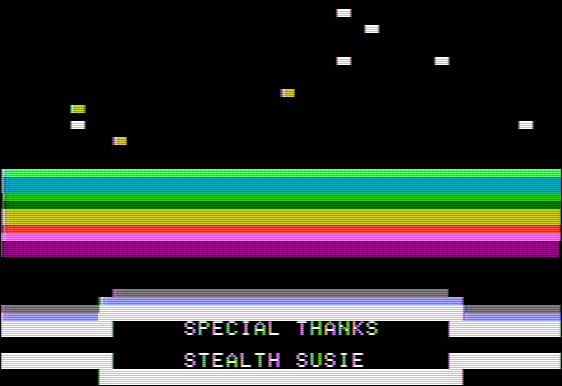
\includegraphics[width=\columnwidth]{figures/m7_screen2.jpg}
\end{figure}

\begin{figure}
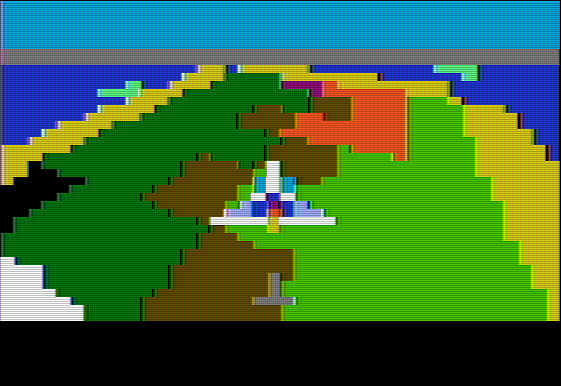
\includegraphics[width=\columnwidth]{figures/m7_screen4.jpg}
\end{figure}

\begin{figure}
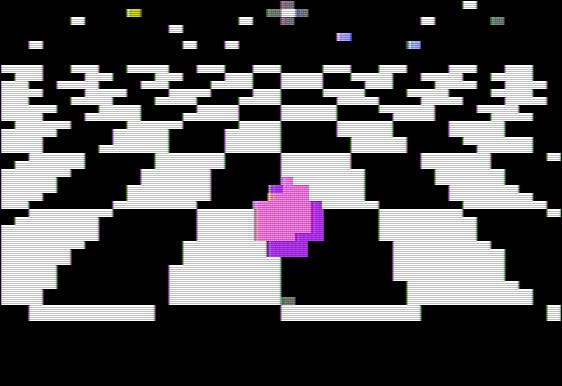
\includegraphics[width=\columnwidth]{figures/m7_screen1.jpg}
\end{figure}

\begin{figure}
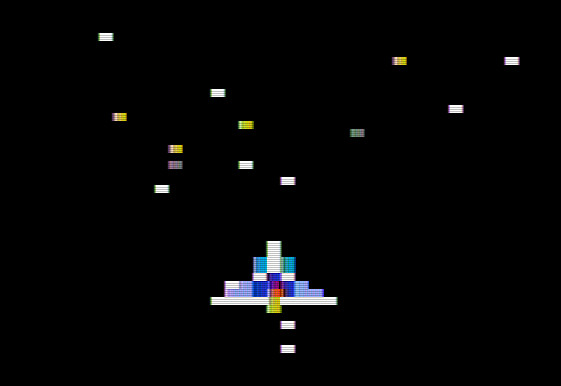
\includegraphics[width=\columnwidth]{figures/m7_screen3.jpg}
\end{figure}

\begin{figure}
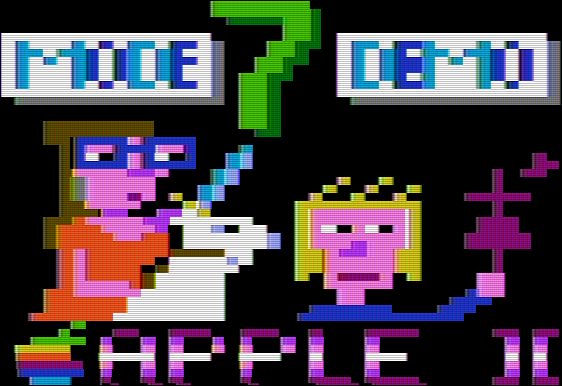
\includegraphics[width=\columnwidth]{figures/mode7_demo_title.png}
\end{figure}

\end{document}
